\chapter{Prezentacja silnika}
\label{chap:engine}

\section{Biblioteki}
\todo[inline]{Myślę, że warto używane narzędzia i~biblioteki opisać w~osobnym rozdziale, a~nie w~podrozdziale ,,Prezentacja silnika''}

\begin{itemize}
\item
  \todo{Wtedy każdy z~tych punktów byłby osobną sekcją}
  \textbf{DirectX 11}\todo{Tu można by dodać cytowanie} jest to biblioteka graficzna wykorzystywana głównie do tworzenia gier komputerowych (np. Baldur's Gate 3, Wiedźmin 3) lub innych aplikacji graficznych. Biblioteka została stworzona w 2009 roku przez firmę Microsoft. Dostępna jest tylko na komputerach z systemem \todoarea{,,Windows'' lub ,,MS Windows''}{windows} i konsolach Xbox. \todo{Nowy akapit (jeśli sekcja)}W silniku wykorzystywana jest do grafiki poprzez shadery \footnote{Shader to program działający na karcie graficznej\todo[inline]{Jak treść zostanie rozbudowana, to to nie musi być footnote}} takie jak: compute shader, pixel shader i vertex shader.
    \item \textbf{Win32} jest to interfejs programistyczny systemu Windows. Zawiera w sobie funkcje umożliwiające działanie programów w systemie. Okno prezentowanego silnika zostało stworzone za pomocą tej biblioteki.\todo{Jak ImGui ma się do Win32?}
    \item \textbf{ImGui}\todo{Tu należy dodać cytowanie} biblioteka wykorzystywana do tworzenia interfejsu użytkownika. Napisana jest w myśl paradygmatu "Immediate Mode GUI" (IMGUI), który głównie polega na tym, że interfejs jest cały czas odświeżany, nie przechowuje on stanu między klatkami przez co jest zawsze zsynchronizowany z danymi. Biblioteka ta jest również łatwiejsza w obsłudze niż np. biblioteka \todoarea{Qt}{QT}. 
    \item \textbf{Assimp}\todo{Tu albo trochę dalej należy dodać cytowanie} Open Asset Import Library jest to biblioteka umożliwiająca łatwe ładowanie modeli 3D w różnych formatach np. obj, glb.\todo{Z jakich formatów korzysta program?} Napisana jest w języku \todoarea{Albo C, albo C++}{C/C++}.
    \item \textbf{Stb\_Image}\todo{Tu należy dodać cytowanie} biblioteka wykorzystywana do ładowania tekstur w \todoarea{a w jakich formatach są używane?}{różnych formatach}.\todo{W jakim języku napisana?}
\end{itemize}
\todo[inline]{Brakuje informacji o~tym, skąd zostały wzięte modele 3D, i~skąd zostały wzięte używane tekstury.}
\item[inline]{Może warto napisać z~jakiego IDE (i~z~jakich pluginów) się korzystało, i~jak rozwiązano zależności i/lub budowanie: premake, CMake, MSBuild, Conan, Build2, vcpkg, Meson, Bazel, make/Makefile.}

\begin{figure}[htbp]
    \centering
    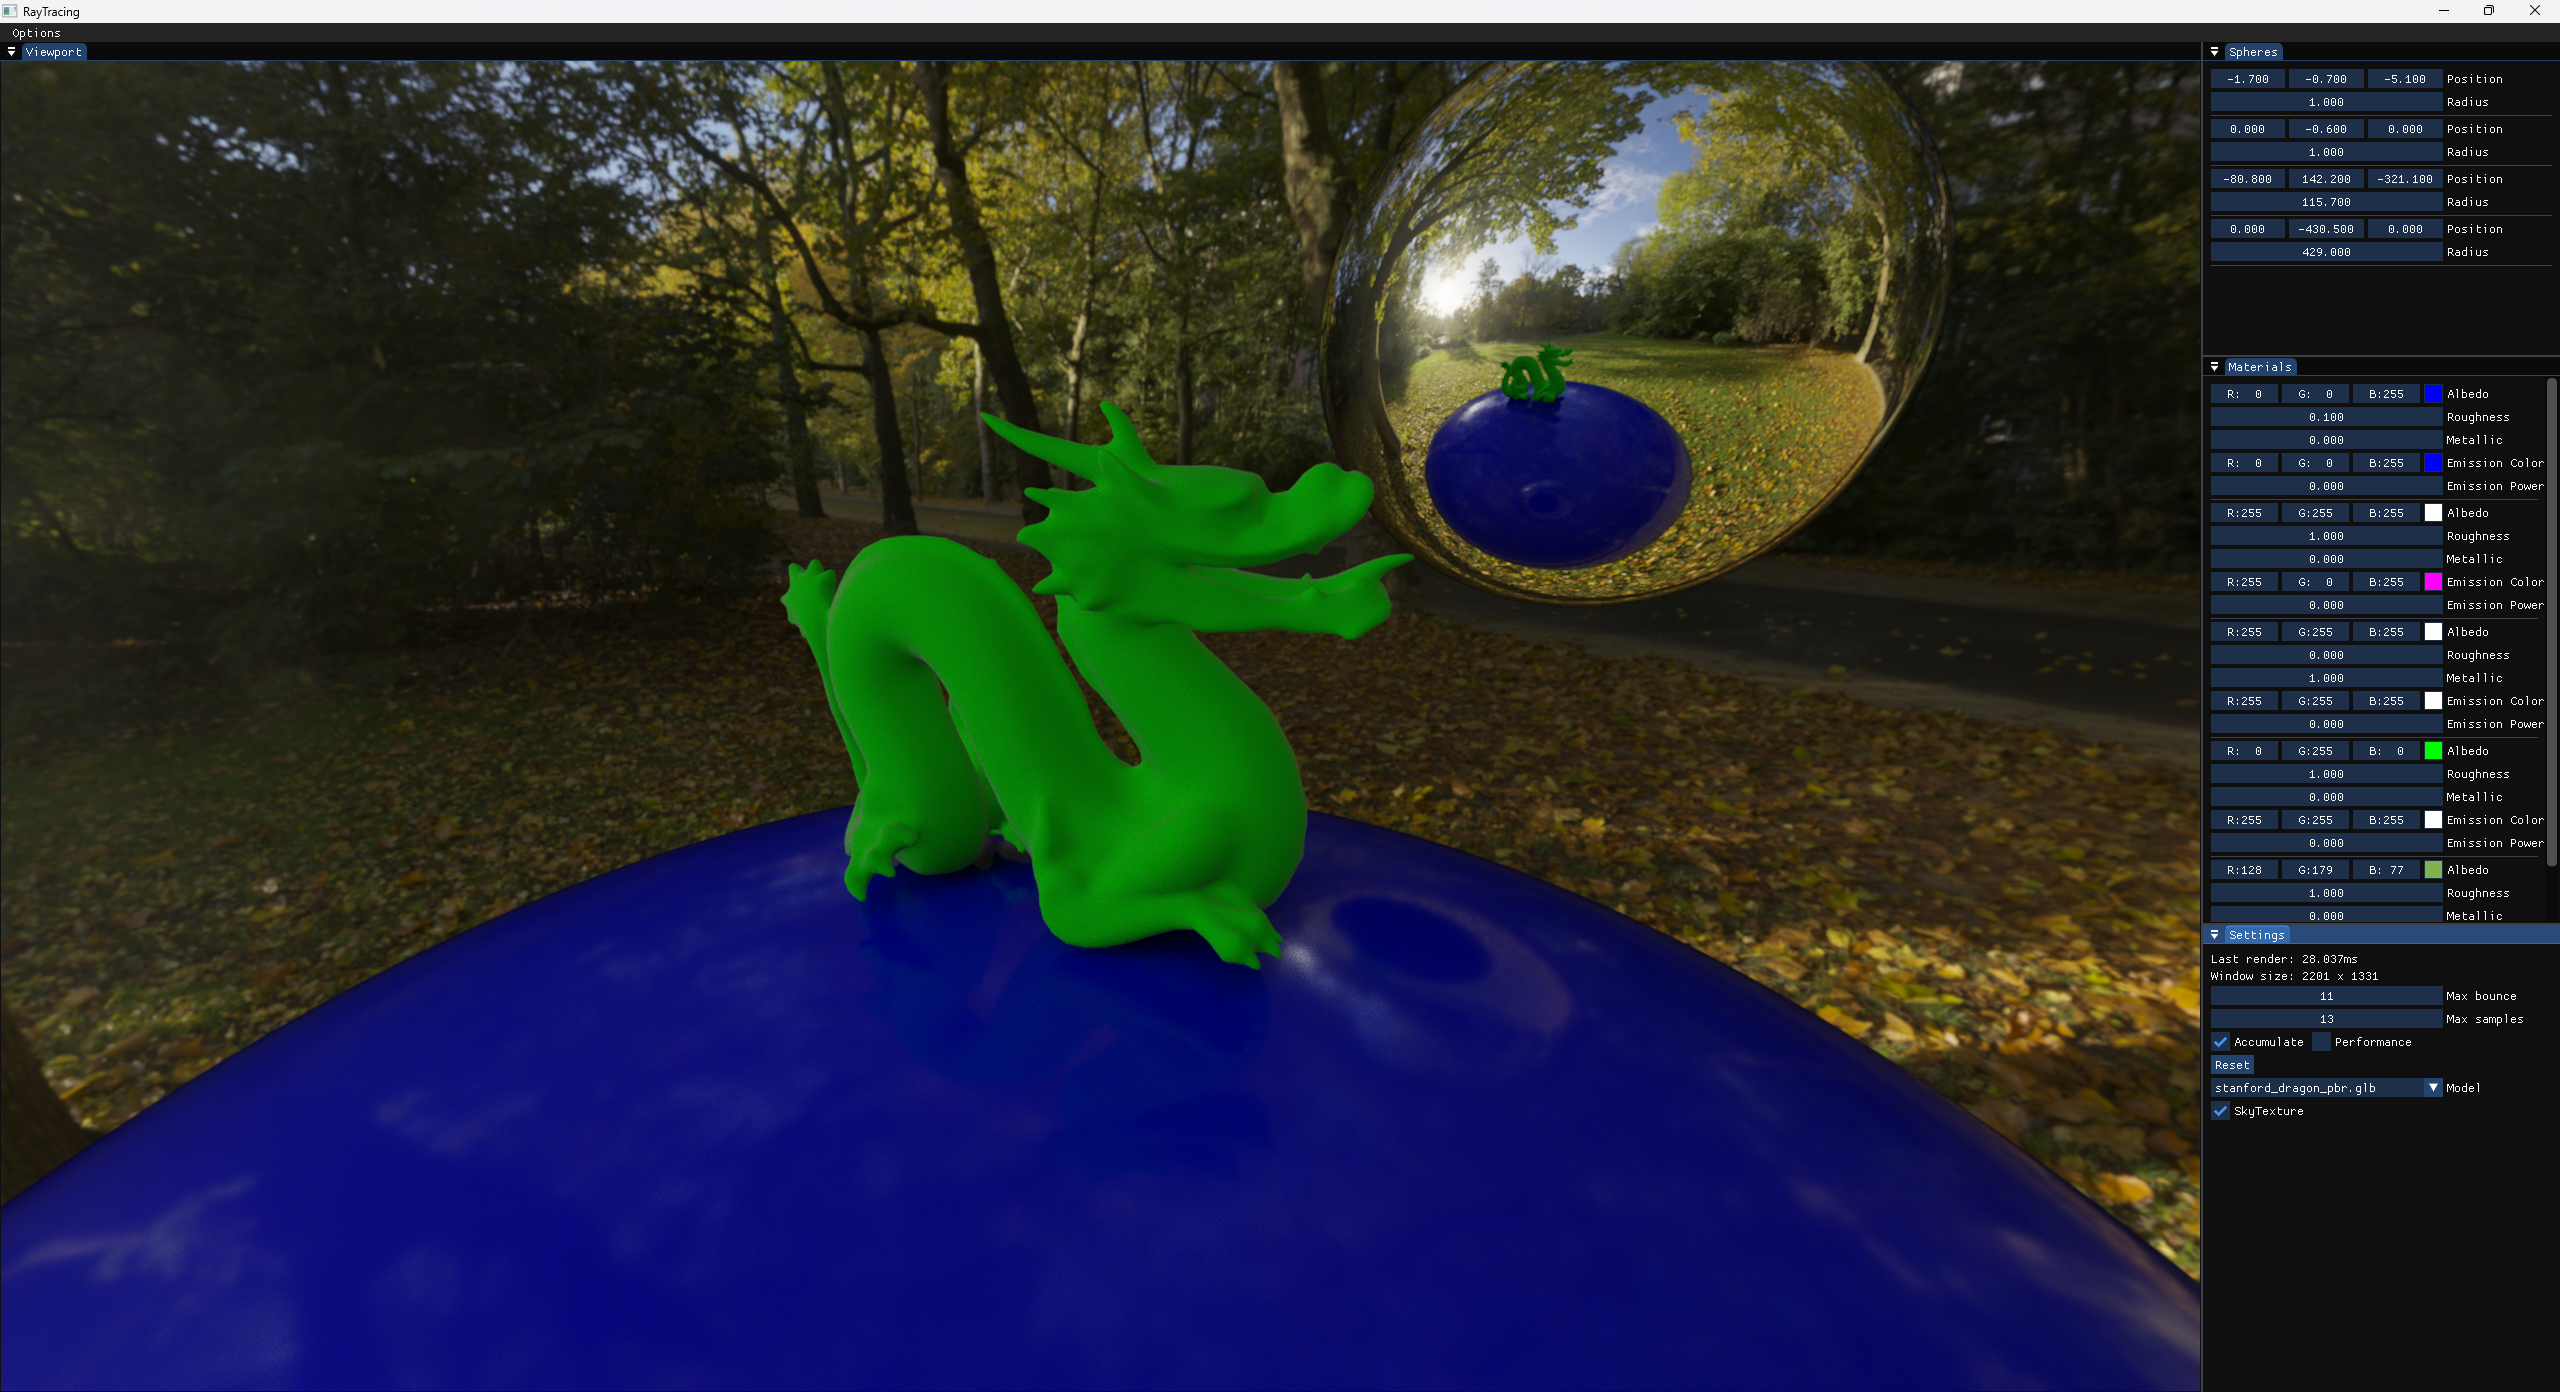
\includegraphics[width=1\textwidth]{Interfejs} 
    \caption{
      Zdjęcie przedstawia interfejs silnika.
      \todo[inline]{Raczej: ,,Interfejs stworzonego w~ramach pracy silnika ray-tracing''}
      \todo[inline]{To nie częścią opisu narzędzi i~technologii}
    }
    \label{fig:interfejs}
\end{figure}

\section{Elementy silnika}

\begin{figure}[H]
    \centering
    \includegraphics[width=1\textwidth]{SchematSilnika} 
    \caption{Schemat silnika.}
    \label{fig:uml}
\end{figure}

\section{Opis potoku graficznego}

Potok graficzny (ang. \textit{graphics pipeline} lub \textit{rendering pipeline}) jest to sekwencja kroków które należy wykonać aby otrzymać obraz na ekranie. Na rysunku \ref{fig:pipeline} widoczny jest cały potok graficzny używany w DX11. Strzałki oznaczają przepływ danych np. vertex shader otrzymuje dane z fazy Input assembler, wykonuje na nich swoje obliczenia i przekazuje dalej do hull shadera. 

\begin{figure}[H]
    \centering
    \includegraphics[width=0.8\textwidth]{RenderingPipeline} 
    \caption{Zdjęcie przedstawia potok graficzny w DirectX 11. \cite{dx11}}
    \label{fig:pipeline}
\end{figure}

Najważniejszymi shaderami w potoku są vertex shader i pixel shader (pixel shader czasem nazywany jest fragment shaderem np. w openGL). 
\begin{itemize}
    \item \textbf{Vertex shader} zajmuje się przekształcaniem samych wierzchołków np. nakłada przekształcenia. Vertex shader wykonuje się dla każdego przekazanego wierzchołka na karcie graficznej przez co jest bardzo szybki \cite{dx11}.
    \item \textbf{Pixel shader} zajmuje się kolorem danego piksela, to tutaj wykonuje się kod implementujący np. oświetlenie w scenie.
\end{itemize}

Poza potokiem graficznym znajduje się compute shader. Compute shader jest shaderem ogólnego przeznaczenia, można w nim implementować np. ray tracing.


W prezentowanym silniku potok graficzny wygląda następująco:

\begin{center}
    Compute shader $\rightarrow$ (Vertex Shader $\rightarrow$ Pixel Shader) $\rightarrow$ ImGui $\rightarrow$ Prezentacja w oknie
\end{center}

W compute shaderze zaimplementowana jest cała logika ray tracingu, shader zapisuje wyniki obliczeń jako kolor RGBA do tekstury 2D. Następnie tekstura przyjmowana jest jako wejście do pixel shadera, który zamienia wejściową teksturę mającą format R16G16B16A16 (16 bitów na piksel) na format standardowy R8G8B8A8 (8 bit na piksel). 

Silnik wykonuje tzw. rendering to texture, jest to technika polegająca na zapisaniu całej sceny do tekstury, która zostaje nałożona na wybrany obiekt. Standardowym podejściem jest teksturowanie prostokąta, który ma taki sam rozmiar jak okno aplikacji, innym szybszym sposobem jest narysowanie dużego (wykraczającego poza ekran programu) trójkąta \cite{triangle,triangle2}, takie podejście sprawia, że vertex shader musi przekształcić tylko 3 wierzchołki, a nie 4 jak przy prostokącie (przy użyciu tzw index buffer nie trzeba powtarzać wierzchołków).


\section{Implementacja algorytmów}

W tej części przedstawione zostaną implementacje wcześniej omówionych algorytmów. Wszystkie napisane są w języku HLSL (ang. High-Level Shader Language).


\subsection{Implementacja testu przecięcia promień-sfera}

\lstset{
    language=C++,
    basicstyle=\fontsize{11}{13}\ttfamily,
    keywordstyle=\color{blue}\bfseries,
    commentstyle=\color{green},
    stringstyle=\color{orange},
    morekeywords={float4, float3, float2, float4x4, sampler2D, texture2D, lerp},
    numbers=left,
    numberstyle=\tiny\color{gray},
    frame=tb,
    breaklines=true
}


\begin{lstlisting}[label={lst:hlslTriangle}]
    
    float SphereIntersection(Ray ray, Sphere sphere)
    {
        float3 spherePosition = float3(sphere.position.xyz);
        float3 oc = ray.origin - spherePosition;
    
        float a = 1; //dot(ray.direction, ray.direction);
        float b = 2.0 * dot(ray.direction, oc);
        float c = dot(oc, oc) - sphere.radius * sphere.radius;
    
        float discriminant = b * b - 4.0f * a * c;
    
        if (discriminant < 0.0f)
        {
            return -1.0f;
        }
    
        float t1 = (-b - sqrt(discriminant)) / (2.0f * a);
        float t2 = (-b + sqrt(discriminant)) / (2.0f * a);
    
        if (t1 > 0.0f && t2 > 0.0f)
        {
            return min(t1, t2);
        }
        else if (t1 > 0.0f)
        {
            return t1;
        }
        else if (t2 > 0.0f)
        {
            return t2;
        }
        else
        {
            return -1.0f;
        }
    }

\end{lstlisting}

Zmienna $a$ ma wartość $1$, ponieważ $ray.direction$ jest wektorem znormalizowanym, iloczyn skalarny dwóch tych samych znormalizowanych wektorów wynosi $1$. 


\subsection{Implementacja testu przecięcia promień-trójkąt}

\begin{lstlisting}
TriangleHit TriangleIntersection(Ray ray, Triangle tri)
{
    TriangleHit result;
    result.t = -1.0f;
    result.u = -1.0f;
    result.v = -1.0f;
    float3 e1 = tri.v2.xyz - tri.v1.xyz;
    float3 e2 = tri.v3.xyz - tri.v1.xyz;
    
    float3 q = cross(ray.direction, e2);
    float a = dot(e1, q);
    
    if (a > -EPSILON && a < EPSILON)
    {
        return result;
    }
    
    float f = 1 / a;
    
    float3 s = ray.origin - tri.v1.xyz;
    float u = f * dot(s, q);
    
    if (u < 0.0f)
    {
        return result;
    }
    
    float3 r = cross(s, e1);
    float v = f * dot(ray.direction, r);
    
    if (v < 0.0f || u + v > 1.0f)
    {
        return result;
    }
    
    float t = f * dot(e2, r);
    
    if (t > EPSILON)
    {
        result.t = t;
        result.u = u;
        result.v = v;
        return result;
    }
    return result;
}
\end{lstlisting}

\subsection{Przechodzenie przez drzewo BVH}

\begin{lstlisting}
int stack[32];
int stackPtr = 0;
stack[stackPtr++] = 0;

while (stackPtr > 0)
{
    int nodeIdx = stack[--stackPtr];
    BVHNode node = g_BVHNodes[nodeIdx];
    
    float aabbDist = IntersectAABB(ray, node);
    
    if (aabbDist < 0.0f || aabbDist >= info.hitDistance)
    {
        continue;
    }
    
    if (node.triangleCount > 0)
    {
        for (uint k = 0; k < node.triangleCount; k++)
        {
            int triIdx = g_TriIndexes[node.leftFirst + k];
            Triangle tri = g_Triangles[triIdx];
            
            TriangleHit hit = TriangleIntersection(ray, tri);
            
            if (hit.t < 0.0f)
            {
                continue;
            }
            
            if (hit.t < info.hitDistance)
            {
                info.hitDistance = hit.t;
                info.t = hit.t;
                info.hitPoint = RayAt(ray, hit.t);
                
                float w = 1.0f - hit.u - hit.v;
                
                info.normal = normalize(tri.n1.xyz * w + tri.n2.xyz * hit.u + tri.n3.xyz * hit.v);
                info.objectIndex = triIdx;
                info.materialIndex = 3;
            }
        }

    }
    else
    {
        int leftChild = node.leftFirst;
        int rightChild = node.leftFirst + 1;
        
        if (rightChild < numOfNodes)
        {
            stack[stackPtr++] = rightChild;
        }
        if (leftChild < numOfNodes)
        {
            stack[stackPtr++] = leftChild;
        }
    }
}
\end{lstlisting}

Silnik używa shaderów w wersji 5 (model 5.0), ta wersja nie może używać rekurencji (rekurencja dostępna jest dla shaderów DXR używających wsparcia sprzętowego RTCores \cite{DXR}), dlatego funkcja imituje rekurencje używając "stos". Z rozdziału \ref{chap:optymalizacja} wiadomo, że jeśli $triangleCount > 0$, to wierzchołek jest liściem, po sprawdzeniu wykonuje się standardowy kod sprawdzający przecięcie z trójkątem. Jeśli wierzchołek nie jest liściem, to jego potomków dodaje się do stosu. 

\subsection{Główna logika ray tracingu}

Poniżej fragment funkcji implementującej model oświetlenia opisany w rozdziale \ref{chap:materialy}.

\begin{lstlisting}
    Material material = g_Materials[info.materialIndex];
    
    light += GetEmission(material) * contribution;
    
    ray.origin = info.hitPoint + info.normal * EPSILON;
    
    float3 V = -ray.direction;
    
    float3 Fdielectics = float3(0.04f, 0.04f, 0.04f);
    float3 F0 = lerp(Fdielectics, material.albedo.xyz, material.metalness);
    
    float cosTheta = dot(info.normal, V);
    float3 F = FresnelSchlick(max(cosTheta, 0.0f), F0);
    
    float reflectionChance = max(F.r, max(F.g, F.b));
    float randomValue = RandomFloat(seed);
    float2 xi = float2(RandomFloat(seed), RandomFloat(seed));
    
    if (randomValue < reflectionChance)
    {
        
        float3 H = SampleGGX(xi, info.normal, material.roughness);
        float3 L = reflect(-V, H);
        
        float NdotV = saturate(dot(info.normal, V));
        float NdotL = saturate(dot(info.normal, L));
        float NdotH = saturate(dot(info.normal, H));
        float VdotH = saturate(dot(V, H));
        
        if (NdotL > 0.0f)
        {
            float G = G_Smith(material.roughness, NdotV, NdotL);
            float3 weight = (F * G * VdotH) / max(NdotH * NdotV, EPSILON);
            
            contribution *= weight / reflectionChance;
            ray.direction = L;
        }
        else
        {
            return float3(0, 0, 0);
        }
    }
    else
    {
        if (material.metalness >= 1.0f)
        {
            return light;
        }
        float3 L = normalize(RandomVec3OnUnitHemiSphere(seed, info.normal));
        float NdotL = saturate(dot(info.normal, L));
        
        float3 kd = (1.0f - F) * (1.0f - material.metalness);
        contribution *= (material.albedo.xyz * kd * NdotL * 2.0f) / (1.0f - reflectionChance);
        ray.direction = L;
    }
\end{lstlisting}

Zmienna $contribution$ odpowiada za śledzenie strat energii światła podczas każdego odbicia promienia od powierzchni. Jest związana z zasadą zachowania energii, którą trzeba przestrzegać implementując PBR. Zmienna inicjalizowana jest wartością $1$. 


Zmienna $light$ oznacza zakumulowany kolor dla piksela, końcowy wynik obliczeń dla danej ścieżki.
